\documentclass[11pt,conference]{IEEEtran}
\usepackage[utf8]{inputenc}
\usepackage[english]{babel}
\usepackage{graphicx}
\graphicspath{ {images/} }

\begin{document}

\section{Approach}
Our original plan was to utilize ROS on Linux to interface with the Kinect, but we were unable to get the drivers to work with our model of Kinect and opted instead to use the Kinect SDK for Windows. After analyzing this technology for some time, we decided that the best approach to the problem was to break it down into three smaller subproblems: raw data acquisition, production of models for use with libSVM, and gesture matching. The first two deal with specifying the gestures that were ultimately used in the system, while the last actually recognized them. Each of these subproblems was dealt with by its own program, which we will detail here.
\subsection{Raw Data Acquisition}
The first program gathered joint data from the Kinect and placed it in a file. After initializing the Kinect and setting it up to capture skeleton data, the program entered into a data capture loop. Here, the program waits until it starts receiving meaningful data. Once it does, it outputs the data to a file and to the screen, waits for 200 milliseconds, and repeats the process until 25 frames of data have been captured. The file is formatted with each line containing the frame number, joint number, x coordinate of the joint, y coordinate, and z coordinate.

\begin{figure}[h]
\caption{A portion of the raw data file.}
\centering
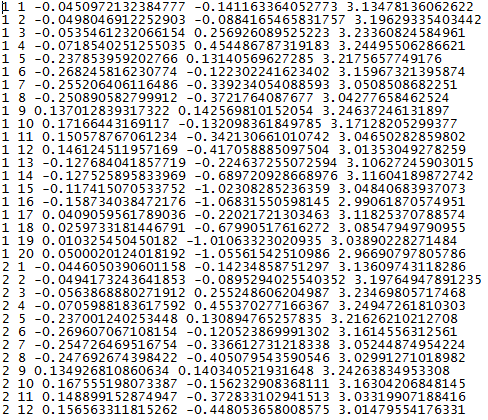
\includegraphics[width=\linewidth]{raw_data}
\end{figure}

Because all of our gestures are static, 25 frames seemed like a good amount of data to collect. It is small enough that the actor does not have to stand for too long, yet large enough to capture some good data. In retrospect, it may have helped to improve our accuracy if we had experimented with which number of frames gave us the best accuracy.

The Kinect does not always produce good data; on occasion, the skeleton will appear ``jittery." To help rectify this, we wait 200 milliseconds between frames. This reduces some of that jitter, which important for our training set in particular. It also allows the program operator to quickly browse over some of the incoming data to ensure that it appears to be meaningful.

\subsection{Production of Models For Use With LIBSVM}
The second program processed the raw data that was read in from the kinect using a simple star skeleton approach. The processed data was then read into libSVM to produce a model. This model could then be used to predict gestures.

To process the data for libSVM we had to first calculate the angles and distances between the center reference point and each of the five points on the star skeleton. After calculating the distance and angles, we stored the data into histograms made up of a set number of bins.

\begin{figure}[h]
\caption{A portion of the processed data file.}
\centering
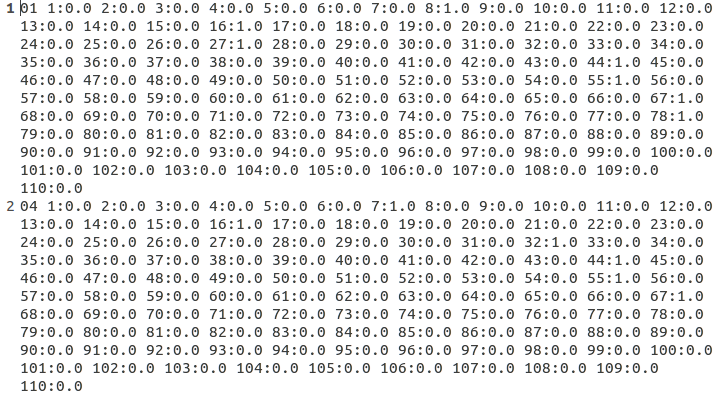
\includegraphics[width=\linewidth]{processed_data}
\end{figure}

After the data was processed it was stored in a file. This file was then read directly into libSVM to produce the model for our gestures. 

\subsection{Gesture Matching}
The third program was used to recognize gestures. Upon initialization, the model created from the second program is loaded into libSVM. Then, for each frame of data produced by the Kinect, our program loads each joint into a data structure that specifies its position. This joint is added to a list that contains all joint data for that particular frame. This list is then added to another list, which is a collection of joint data for a series of frames. Once the size of the latter list reaches 25 (i.e., 25 frames have been analyzed), we run some code from program 2 on it to place the data into a histogram, which is then loaded into libSVM for analysis. Each bin of the histogram is numbered and has a value. To allow libSVM to interpret the data, we paired the number of the bin with the value inside it; this pair is referred to as a node. Once a full set of nodes has been obtained, the program uses the model it loaded earlier to make a ``prediction" as to what action was performed in the 25 frames being analyzed. The prediction comes in the form of a number corresponding to the gesture being recognized. At this point, we use a switch statement to detect the gesture and send the proper keyboard signals to the window in focus.
\end{document}